\chapter{Features}\label{ch:features}
One of the greatest challenges of Vulkan is to offer a high hardware performance, with the lowest consumption possible
and reducing the overhead. Nowadays, mobile devices have the chance of running games with a great graphical quality.
One method that is employed is to reduce the use of the \gls{cpu}. This reduction is performed by a reduction in the
number of delegated tasks, instead the responsibility of the \gls{gpu} is increased: use of batch tasks in the
\gls{gpu}, exclusive use of the cpu for rendering and computation.

Reaching to all devices is other of the main objectives. Vulkan LunarG implementation is available from Windows 7 to
Windows 10, Tizen, GNU\/Linux and Android. The \gls{sdk} is can be installed in both Windows and GNU\/Linux desktop
environments. In MacOS is being developed by third parties for achieving the execution of Vulkan applications. \emph{The
Brenwill Workshop} is a development company specialized on graphics software. They have proposed to create a middleware
between the OpenGL and Metal \gls{api} implementations for getting the support of Vulkan on MacOS and iOS. The solution
is called Molten, and it is part of an available graphic development framework.

Vulkan implements several improvements at technical level, which are a good reason for being the best successor of
OpenGL:
\begin{itemize}
    \item Native muticore \gls{cpu}s scaling support.
    \item Use of intermediate binary format called SPIR-V: Vulkan generates its own code for generating shaders, so
    that the drivers do not require the development of a compiler for being able to render them. As the shaders are
    compiled, a higher range of shaders can be used per scene. The driver just is in charge of optimize and generate
    the final compiled code.
    \item Unified management of computing kernels and graphical shaders: both \gls{api} are mixed that, until now, were
    separated.
    \item Oriented to objects, there is no global state.
    \item States are not tied into a context, they are cached in a buffer.
    \item Multithreading support.
    \item More control over memory and synchronization.
\end{itemize}

There are features that have been proposed, but will be implemented in the future. For instance, providing support to
multiple \gls{gpu}s of different model. The need of using \gls{sli} for being able to use several graphical cards at
the same time.

On the figure \ref{fig:comparison_opengl_vulkan} the existing differences between the two \gls{api} can be appreciated
more graphically. As you may notice among the features of Vulkan, a closest access to the hardware from the applications
has been attempted. Thanks to this, the need of a huge error and memory management is removed. Only a intermediate
language is employed for using shaders (SPIR-V), and the \gls{api} is the same for developing on both mobile
applications and desktop applications.

Knowing all these information could be concluded that Vulkan increases the work load that the developers already have.
However, things are not as they appear. Vulkan can be applied at three different levels:

\begin{enumerate}
    \item Use directly all these features for having a full control over the engine.
    \item Use and share libraries and layers for accelerating the development process.
    \item Use already existing and optimized engines over the Vukan \gls{api}.
\end{enumerate}

The first option is the less frequent since developers have to start from scratch. But it could be a good option for
making good benchmarks. Khronos expects the second option to be a rich area of innovation among the community and
companies. As the libraries can be published as little bundles, they could be shared as OpenSource that require
improvements and updates. The last option could be the most tentative considering that the hard work has already
done by industry giants, developers have only to pay some royalties to the propietaries of the engine; for instance
Unity Engine.

On the figure \ref{fig:vulkan_ecosystem} can be appreciated how the Vulkan architecture is distributed. As explained,
the Vulkan implementation is placed in a lower level that the game engine. It is located over the hardware so that
many of its features can be exploded directly. An interface is set up for implementing other tools and frameworks
joined together with Vulkan in the future.

\begin{figure}[t]
	\begin{center}
		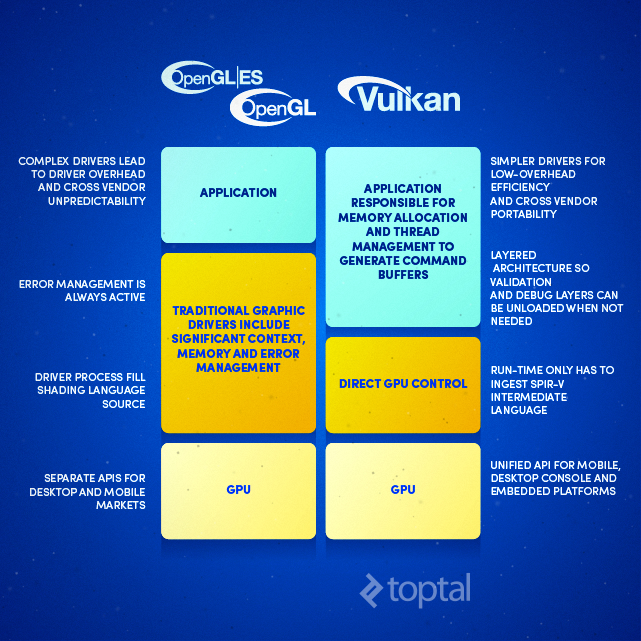
\includegraphics[scale=0.3]{comparison-opengl_and_vulkan}
		\caption{Features of OpenGL and Vulkan comparison}
		\label{fig:comparison_opengl_vulkan}
	\end{center}
\end{figure}
\begin{figure}[t]
	\begin{center}
		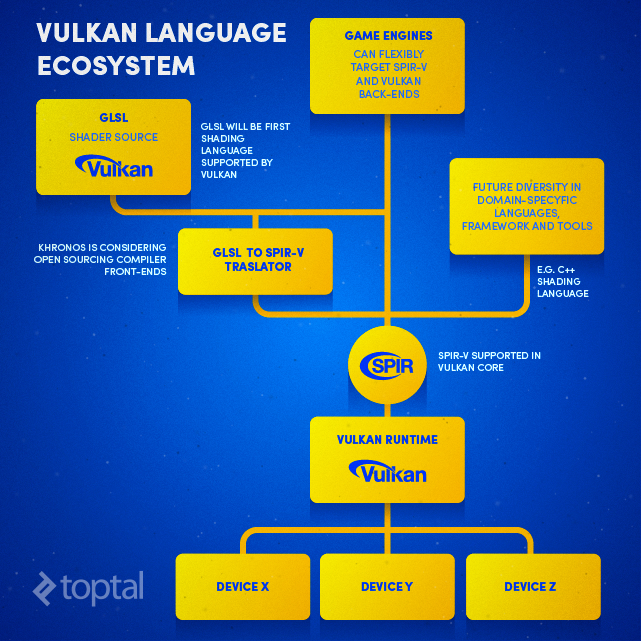
\includegraphics[scale=0.3]{ecosystem-vulkan}
		\caption{Vulkan Ecosystem}
		\label{fig:vulkan_ecosystem}
	\end{center}
\end{figure}
